\documentclass[a4paper,12pt]{report}
\usepackage[left=2.5cm,right=2.5cm,top=3cm,bottom=2.5cm]{geometry}
\usepackage{fancyhdr}
\usepackage{etoolbox}
\usepackage{titlesec}
\usepackage{titling}
\usepackage{pgfplots}

\pagestyle{fancy}
\fancyhf{}
\fancyhead[L]{UTN-FRC}
\fancyhead[C]{Física Electrónica: Radiación Térmica}
\fancyhead[R]{2R3}
\renewcommand{\headrulewidth}{0.4pt}
\fancyfoot[C]{\vfill\thepage}
\setlength{\headwidth}{\textwidth} % Hace que el ancho del encabezado coincida con el ancho del texto
\setlength{\headheight}{15pt}  % Ajusta la altura del encabezado
\setlength{\headsep}{20pt}     % Ajusta la separación entre el encabezado y el contenido

\usepackage{titlesec}
\titleformat{\chapter}[display]
  {\normalfont\Large\bfseries}{}{0pt}{}
\titlespacing*{\chapter}{10pt}{-45pt}{10pt}

\usepackage{etoolbox} 
\makeatletter
\patchcmd{\chapter}{\thispagestyle{plain}}{\thispagestyle{fancy}}{}{} %Muestra encabezado en las paginas con \chapter
\makeatother

\titleformat{\chapter}[display]
  {\normalfont\bfseries}{}{0pt}{\huge}
\titlespacing*{\chapter}{0pt}{-30pt}{20pt}

\DeclareMathSizes{12}{13}{6}{5}

\title{%
  \fontsize{25}{0}\selectfont Universidad Tecnológica Nacional \\
  \fontsize{22}{30}\selectfont Física Electrónica \\
  \fontsize{18}{25}\selectfont TPL1: Radiación térmica
}
\author{
Franco Palombo - 401910\\
Gaston Grasso - 401892\\
Ignacio Gil - 401891\\
Luciano Cortesini - 402719\\
}
\date{3 / 10 / 2024}

\begin{document}

\maketitle

\chapter{Introducción}
  El fenómeno de la radiación es la propagación de energía en forma de ondas electromagnéticas o partículas subatomicas
  que viajan a través del vació o de un medio en especifico.\\

  Existen múltiples tipos de radiación, pero para el enfoque de este trabajo practico, se va a experimentar con la
  radiación térmica, como puede ser la emitida por cualquier cuerpo que se encuentra a una temperatura mayor a 0ºK.
  Este tipo de radiación es denominada radiación térmica. Es producto del movimiento térmico que presentan las
  partículas cargadas presentes en la materia. La intensidad de esta radiación depende de la temperatura de la materia
  o el cuerpo y de la longitud de onda que se considere.\\

  Todos los cuerpos emiten energía y a su vez la absorben de sus inmediaciones. Cuando se alcanza el equilibrio térmico,
  la velocidad de emisión y absorción son iguales. La materia en estado condensado (sólido o líquido) emite un espectro
  continuo de radiación. Este espectro depende solamente de la temperatura.\\

  La radiación por unidad de área se puede calcular de la siguiente forma:
  \begin{equation}
    R = e \sigma T^4
  \end{equation}

  Donde $e$ es el poder emisivo o emisividad relativa a un cuerpo negro, $\sigma$ es la constante de Stefan-Boltzmann y
  $T$ la temperatura en el instante de tiempo dado en grados kelvin.\\

  Los cuerpos pueden ser emisores de radiación o receptores de radiación. En ambos casos, las cantidades son iguales,
  pero opuestas. Esto es debido a la reciprocidad, un fenómeno que establece que la razón de emisión de radiación
  electromagnética de un cuerpo a una frecuencia dada, va a ser la misma a la que el cuerpo pueda absorber.\\

  Para cuerpos emisores, la radiación emitida, puede propagarse en cualquier dirección en cualquiera
  de sus superficies o caras. La emisividad de un cuerpo es la razón entre la intensidad emitida por la
  superficie en una dirección particular y la intensidad que sería emitida por un cuerpo negro a la misma temperatura y
  longitud de onda.\\

  Diferentes cuerpos emiten radiación térmica en diferentes formas. Todos expulsan calor en forma de radiación térmica,
  pero también emiten radiación en el espectro de la luz. Según el material y su temperatura, la radiación en el
  espectro de la luz aumenta o disminuye de intensidad y longitud de onda. Todos los materiales a una
  temperatura menor de 798ºK emiten luz infrarroja. Cuando se supera este umbral, en algunos materiales, suficiente de
  la radiación infrarroja es emitida como para que se empiece a percibir luz visible. De aquí se puede generar un
  espectro de luz que relaciona la temperatura de un material dado y la longitud de onda de la luz que emite.\\\\\\\\
  \begin{figure}[h!]
    \centering
    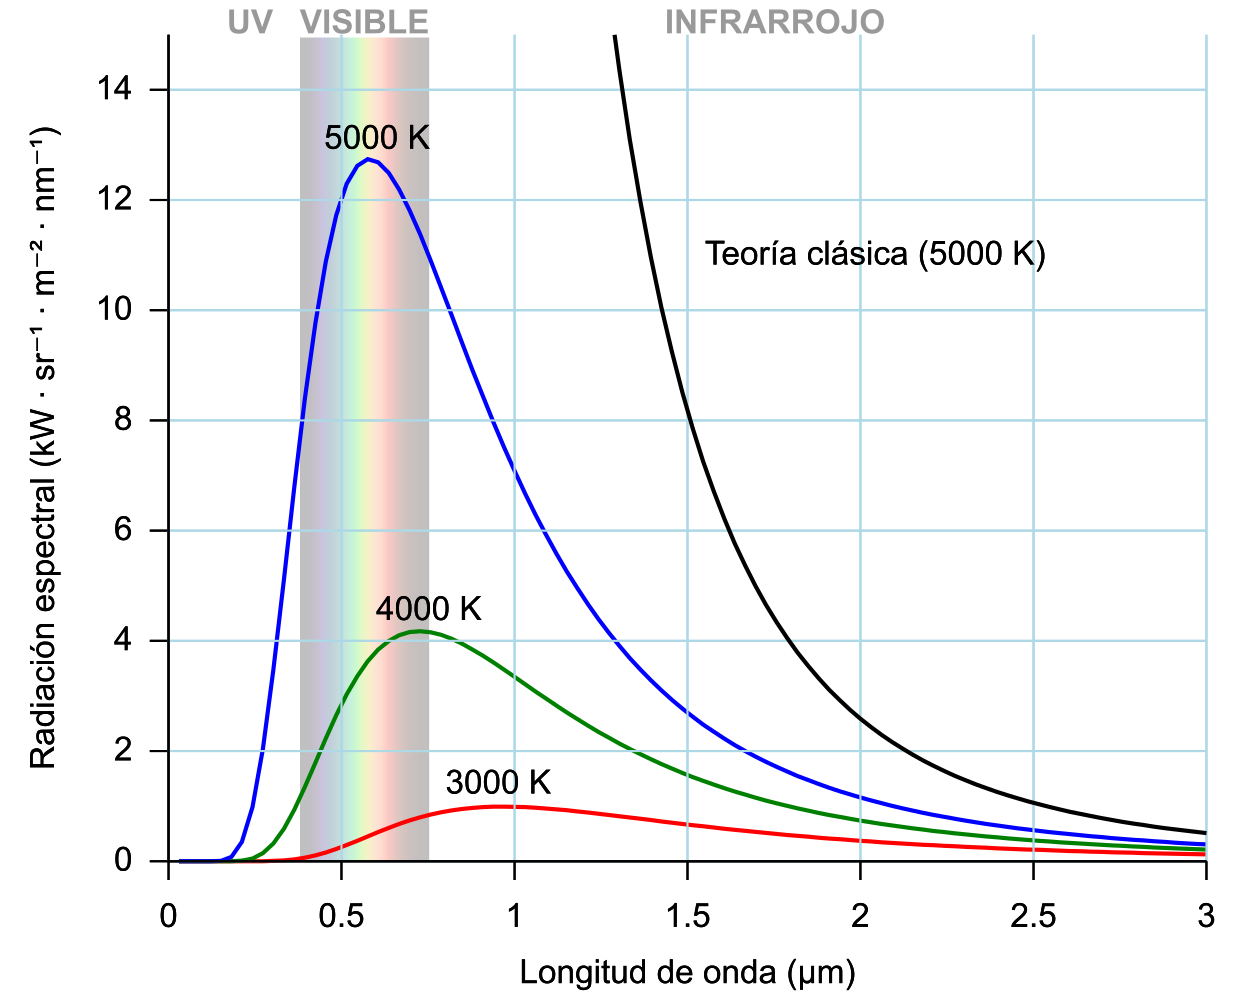
\includegraphics[width=\linewidth]{images/img1.png}
  \end{figure}

  Existe un tipo de cuerpo, cuyas capacidades de emisión y absorción son ideales. Este cuerpo, denominado cuerpo negro,
  esta caracterizado por permitir el paso de todos las ondas electromagnéticas, independientemente de su longitud de
  onda o su dirección. También, no hay superficie que pueda emitir mas radiación que la de un cuerpo negro en las
  mismas condiciones de temperatura y longitud de onda.\\

  Habiendo presentado estos conceptos, se procede a presentar las experiencias de laboratorio.

\chapter{Experiencia de laboratorio}
  Esta experiencia consta en la utilización del cubo de Leslie, un dispositivo que contiene en su interior una fuente
  de radiación térmica en forma de una bombilla incandescente. Una caja metálica, colocada sobre la bombilla, se pone
  en contacto con diferentes tipos de materiales, para probar dos propiedades de los mismos:
  \begin{itemize}
    \item Capacidad de emisión
    \item Capacidad de absorción
  \end{itemize}

  Estas propiedades permiten caracterizar diferentes materiales como aislantes o conductores térmicos, y dependiendo de
  diferentes propiedades físicas, se los puede emplear como capas protectoras del calor o instrumentos de dispersión de
  calor.\\

  Para poder caracterizar los materiales, se empleo un dispositivo que permite medir la temperatura por un medio de
  contacto físico (termistor), y otro dispositivo que permite medir la radiación que emite un cuerpo, por medio de un
  sensor de estado solido que reacciona con la longitud de onda de la banda infrarroja. Ambos dispositivos convierten
  magnitudes físicas en magnitudes eléctricas, específicamente señales de voltaje. Estos voltajes son leídos con un
  dispositivo llamado multimetro. El termistor, por cada grado kelvin, en sus bornes genera 20mV de diferencia de
  potencial, y el medidor de radiación térmica, por cada mW de radiación medido, genera 22mV en sus bornes.

  \section{Radiación en función de la temperatura}

  \begin{center}
    \begin{tikzpicture}
        \begin{axis}[
          title={Aluminio},
          ylabel={Radiación (mW)},
          xlabel={Temperatura (°C)},
          width=11cm,
          height=8cm,
          yticklabel style={/pgf/number format/fixed,/pgf/number format/precision=3},
          ytick distance = 0.01,
          grid=major,
        ]
        \addplot coordinates {
          (67.5,0.136) (67.3,0.132) (66.2,0.127) (63.1,0.114) (60.2,0.1) (58.3,0.091) (57,0.086)
        };
        \end{axis}
    \end{tikzpicture}
  \end{center}

  \begin{center}
    \begin{tikzpicture}
        \begin{axis}[
          width=11cm,
          height=8cm,
          xlabel={Temperatura (°C)},
          ylabel={radiaciom(mW)},
          title={Bronce},
          ytick distance = 0.01,
          grid=major,
        ]
        \addplot coordinates {
          (65,0.145) (64,0.132) (63,0.132) (62,0.127) (61,0.123) (60,0.118) (59,0.109) (58,0.105) (57, 0.1)
        };
        \end{axis}
    \end{tikzpicture}
  \end{center}

  \begin{center}
    \begin{tikzpicture}
        \begin{axis}[
          width=11cm,
          height=8cm,
          xlabel={Temperatura (°C)},
          ylabel={Radiaciom(mW)},
          title={Plomo},
          ytick distance = 0.01,
          grid=major,
        ]
        \addplot coordinates {
          (63,0.227) (62,0.214) (61,0.205) (60,0.2) (59,0.195) (58,0.186) (57,0.173) (56,0.168) (55,0.164)
        };
        \end{axis}
    \end{tikzpicture}
  \end{center}

  \begin{center}
    \begin{tikzpicture}
        \begin{axis}[
          width=11cm,
          height=8cm,
          xlabel={Temperatura (°C)},
          ylabel={Radiaciom(mW)},
          title={Cobre},
          ytick distance = 0.01,
          grid=major,
        ]
        \addplot coordinates {
          (63,0.236) (62.3,0.227) (61.5,0.223) (60.5,0.214) (59.9,0.205) (58.9,0.2) (58,0.191)
        };
        \end{axis}
    \end{tikzpicture}
  \end{center}

  \begin{center}
    \begin{tikzpicture}
        \begin{axis}[
          width=11cm,
          height=8cm,
          xlabel={Temperatura (°C)},
          ylabel={Radiación (mW)},
          title={Aluminio Anodizado},
          ytick distance = 0.01,
          grid=major,
        ]
        % Primera función
        \addplot coordinates {
          (65,0.250) (64,0.241) (63,0.232) (62,0.223) (61,0.214) (60,0.205) (59,0.2) (58,0.191) (57,0.182)
        };
        \end{axis}
    \end{tikzpicture}
  \end{center}

  \begin{center}
    \begin{tikzpicture}
        \begin{axis}[
          width=11cm,
          height=8cm,
          xlabel={Temperatura (°C)},
          ylabel={Radiación (mW)},
          title={Superposición},
          grid=major,
          ytick distance = 0.02,
          yticklabel style={/pgf/number format/fixed,/pgf/number format/precision=3},
          legend style={
            at={(0.5,-0.25)}, % Cambia la posición a bajo el gráfico
            anchor=north, % Ancla al centro norte de la leyenda
            legend columns=2, % Número de columnas en la leyenda
            },
        ]
        \addplot[black,mark=*] coordinates{
          (65,0.250) (64,0.241) (63,0.232) (62,0.223) (61,0.214) (60,0.205) (59,0.2) (58,0.191) (57,0.182)
        }; \addlegendentry{Aluminio anodizado}

        \addplot[blue,mark=*] coordinates{
          (67.5,0.136) (67.3,0.132) (66.2,0.127) (63.1,0.114) (60.2,0.1) (58.3,0.091) (57,0.086)
        }; \addlegendentry{Aluminio}

        \addplot[red,mark=*] coordinates{
          (65,0.145) (64,0.132) (63,0.132) (62,0.127) (61,0.123) (60,0.118) (59,0.109) (58,0.105) (57, 0.1)
        }; \addlegendentry{Bronce}

        \addplot[orange,mark=*] coordinates{
          (63,0.227) (62,0.214) (61,0.205) (60,0.2) (59,0.195) (58,0.186) (57,0.173) (56,0.168) (55,0.164)
        }; \addlegendentry{Plomo}

        \addplot[green,mark=*] coordinates{
          (63,0.236) (62.3,0.227) (61.5,0.223) (60.5,0.214) (59.9,0.205) (58.9,0.2) (58,0.191)
        }; \addlegendentry{Cobre}
        \end{axis}
    \end{tikzpicture}
  \end{center}

  \section{Radiación en función de la distancia}

  \begin{center}
    \begin{tikzpicture}
        \begin{axis}[
          width=11cm,
          height=8cm,
          xlabel={Distancia (mm)},
          ylabel={Radiación (mW)},
          title={Bronce},
          ytick distance = 0.01,
          yticklabel style={/pgf/number format/fixed,/pgf/number format/precision=3},
          grid=major,
        ]
        \addplot coordinates {
          (0,0.1) (10,0.094) (20,0.089) (30,0.084) (40,0.079) (50,0.071) (60,0.064) (70,0.055) (80,0.046) (90,0.04)
        };
        \end{axis}
    \end{tikzpicture}
  \end{center}

\chapter{Conclusiones}
  Gracias a las experiencias de laboratorio, se determino que todos los cuerpos emiten radiación a temperatura ambiente,
  independientemente del material. Ademas, si calentamos un cuerpo a una temperatura dada, su radiación aumenta de
  manera proporcional a ese aumento.

  Según el tipo de material, y los datos recaudados de cada experiencia, es posible agruparlos en buenos y malos
  conductores térmicos. Esta conductividad térmica, va de la mano con la capacidad de emitir radiación térmica a partir
  de la energía interna acumulada, producto del aumento de temperatura provocado por el cubo de Leslie.

  De acuerdo con los datos obtenidos, se puede observar que el aluminio anodizado es el que mejor disipa calor. En
  contraparte, el aluminio es el que peor lo hace. Esto es deducible gracias a la diferencia en niveles de radiación
  que emiten el uno y el otro, estando a temperaturas similares.

\end{document}
